\documentclass[../main.tex]{subfiles}
\begin{document}
\chapter{Integration}
\section{Integrals as Riemann Sums}
\begin{definition}[Integral]
  The \textit{integral} of a (suitably well-defined) function $f(x)$ is the limit of a sum.
\end{definition}
For example:
\[
  \int_{a}^{b} f(x) \d{x} = \lim_{N \to \infty} \sum_{n=0}^{N - 1} f(x_n)\Delta x
\]
Where $\Delta x = \frac{b-a}{N}$ and $x_n = a + n\Delta x$.

This is the left Riemann sum and is visualised in the following diagram:
\begin{center}
 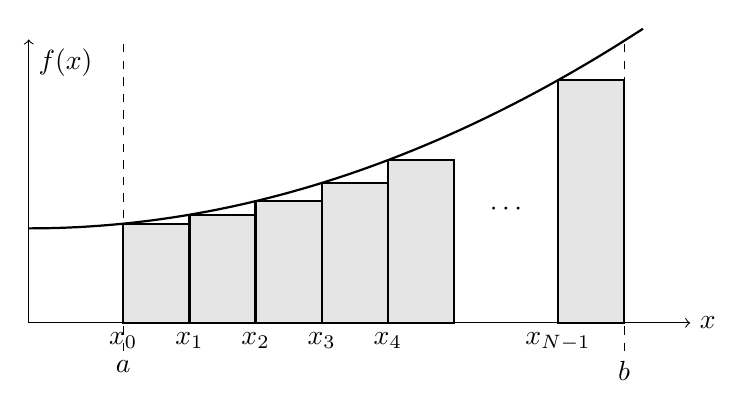
\begin{tikzpicture}[scale=1.2]
  \draw[->] (0,0) -- (7,0) node[right] {$x$};
  \draw[->] (0,0) -- (0,3) node[below right] {$f(x)$};

  \draw[thick, domain=0:6.5, smooth, variable=\x] plot ({\x}, {0.05*\x^2 + 1});

  \node[below] at (1,-0.3) {$a$};
  \draw[dashed] (1,-0.3) -- (1,3);
  \node[below] at (6.3,-0.3) {$b$};
  \draw[dashed] (6.3,-0.3) -- (6.3,3);

  \def\dx{0.7}
  \foreach \i in {0,1,2,3,4} {
    \pgfmathsetmacro{\xleft}{1 + \i*\dx}
    \pgfmathsetmacro{\height}{0.05*\xleft^2 + 1}
    \fill[gray!20] (\xleft,0) rectangle ({\xleft+\dx}, {\height});
    \draw[thick] (\xleft,0) rectangle ({\xleft+\dx}, {\height});
    \node[below] at (\xleft,0) {$x_\i$};
  }

  \node at (5.05,1.2) {$\cdots$};

  \pgfmathsetmacro{\xfinal}{5.6}
  \pgfmathsetmacro{\hfinal}{0.05*\xfinal^2 + 1}
  \node[below] at (\xfinal,0) {$x_{N-1}$};
  \fill[gray!20] (\xfinal,0) rectangle ({\xfinal+\dx}, {\hfinal});
  \draw[thick] (\xfinal,0) rectangle ({\xfinal+\dx}, {\hfinal});
\end{tikzpicture}
\end{center}

\begin{definition}[Riemann Integrable]
  A function $f(x)$ is \textit{Riemann integrable} if the generalised Riemann sum \textbf{does not} depend on how exactly we choose the rectangles in the limit provided all $\Delta x \to 0$ in the limit.

  For example we could have non-uniform $\Delta x$ or evaluate $f$ at the centre or right of each interval.
\end{definition}
To show how this is related to the area under a curve consider a single interval:
\begin{center}
 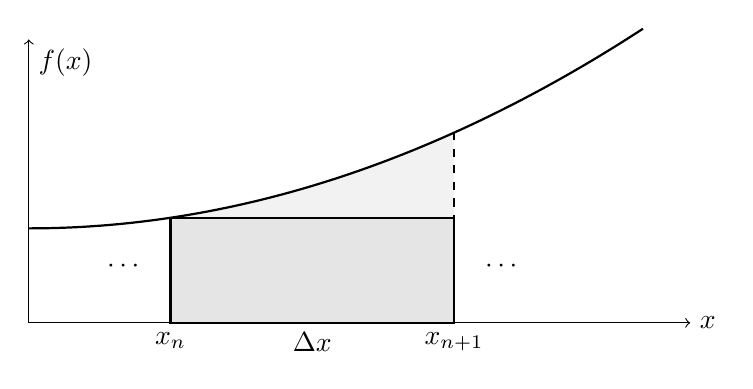
\begin{tikzpicture}[scale=1.2]
  \draw[->] (0,0) -- (7,0) node[right] {$x$};
  \draw[->] (0,0) -- (0,3) node[below right] {$f(x)$};

  \fill [gray!10, domain=1.5:4.5, variable=\x]
    (1.5, 0)
    -- plot ({\x}, {0.05*\x^2 + 1})
    -- (4.5, 0)
    -- cycle;
  \draw[thick, domain=0:6.5, smooth, variable=\x] plot ({\x}, {0.05*\x^2 + 1});

  \pgfmathsetmacro{\height}{0.05*1.5^2 + 1}
  \fill[gray!20] (1.5,0) rectangle (4.5, {\height});
  \draw[thick] (1.5,0) rectangle (4.5, {\height});
  \node at (5,0.6) {$\cdots$};
  \node at (1,0.6) {$\cdots$};
  \node[below] at (1.5,0) {$x_n$};
  \node[below] at (3, 0) {$\Delta x$};
  \node[below] at (4.5,0) {$x_{n+1}$};
  \draw[dashed] (4.5,0) -- (4.5,0.05*4.5^2 + 1);
\end{tikzpicture}
\end{center}
\begin{theorem}[Mean Value Theorem]
  For $f(x)$ continuous, the area under the \textbf{curve} from $x_n$ to $x_{n + 1}$ is:
  \[
    A_n = (x_{n+1}-x_n)f(c_n) = \Delta x f(c_n)
    \label{meanValue}
  \]
  for some $c_n$ with $x_n \leq c_n \leq x_{n+1}$.
\end{theorem}
If $f(x)$ is differentiable, we can use the stronger case of \cref{taylorsThm} (Taylor's Theorem) to write:
\begin{align*}
  f(c_n) &= f(x_n) + O(c_n - x_n) \quad \text{ as } c_n - x_n \to 0 \\
         &= f(x_n) + O(\Delta x) \text{ since $\Delta x \geq c_n - x_n$}
\end{align*}
So we have that:
\[
  A_n = \Delta x f(x_n) + O((\Delta x)^2) \quad \text{ as } \Delta x \to 0
\]
Therefore the total area from $x=a$ to $x=b$ is:
\begin{align*}
  A &= \lim_{N \to \infty} \sum_{n=0}^{N-1} A_n \\
    &= \lim_{N \to \infty} \sum_{n=0}^{N-1} f(x_n) \Delta x + \lim_{N \to \infty} \underbrace{NO\left[\left(\frac{b-a}{N}\right)^2\right]}_{O(1/N)} \\
    &= \int_{a}^{b} f(x) \d{x} + 0
\end{align*}
\section{Fundamental Theorem of Calculus}
\begin{theorem}[Fundemental Theorem of Calculus]
  \label{FTC}
  If
  \[
    F(x) = \int_{a}^{x} f(t) \d{t}
  \]
  then:
  \[
    \deriv{F}{x} = \deriv{}{x}\left(\int_{a}^{x} f(t) \d{t}\right) = f(x)
  \]
\end{theorem}
\begin{proof}
  \begin{align*}
    \deriv{F}{x} &= \lim_{h \to 0} \frac{1}{h} \left[\int_{a}^{x+h} f(t) \d{t} - \int_{a}^{x} f(t) \d{t}\right] \\
                 &= \lim_{h \to 0} \frac{1}{h} \left[\int_{x}^{x+h} f(t) \d{t}\right] \\
                 &= \lim_{h \to 0} \frac{1}{h} \left[hf(c)\right] \text{ with } x \leq c \leq x + h \text{ from \cref{meanValue} (MVT)} \\
                 &= \lim_{h \to 0} [f(x) + O(c-x)] \text{ from \cref{taylorsThm} (Taylor's Theorem)} \\
                 &=\lim_{h \to 0} [f(x) + O(h)] \text{ since $h \geq c-x$} \\
                 &= f(x)
  \end{align*}
\end{proof}
\begin{remark}[Note]
  $F(x)$ is a solution to the differential equation:
  \[
    \deriv{F}{x} = f(x) \text{ with } F(a) = 0
  \]
\end{remark}
\begin{corollary}
  We can swap the limits for:
  \[
    \deriv{}{x}\left(\int_{x}^{b} f(t) \d{t}\right) = -f(x)
  \]
  We can use the chain rule to get:
  \begin{align*}
    \deriv{}{x}\left(\int_{a}^{g(x)} f(t) \d{t}\right) &= \deriv{}{x}F(g(x)) \\
                                            &= \deriv{F}{g} \deriv{g}{x} \\
                                            &= f(g(x)) g'(x)
  \end{align*}
\end{corollary}
\begin{remark}[Notation]
  We denote indefinite integrals as:
  \[
    \int f(x) \d{x} \text{ or } \int_{}^{x} f(x) \d{x}
  \]
  In the latter case, the unspecified lower limit gives rise to the integration constant.
\end{remark}
\section{Integration Techniques}
\subsection{Substitution}
If the integrand contains a function of another function, it might help to substitute for the inner function.
\begin{example}
  Consider:
  \[
    I = \int \frac{1-2x}{\sqrt{x - x^2}} \d{x}
  \]
  Let $u = x - x^2$ so $\deriv{u}{x} = 1 - 2x$.
  So
  \[
    I = \int \frac{\d{u}}{\sqrt{u}} = 2\sqrt{u} + C = 2\sqrt{x - x^2} + C
  \]
\end{example}
\subsubsection{Trig. Substitutions}
\begin{center}
\begin{tabular}{c|c|c}
Identity & Integrand Contains & Subtitution \\
\hline
$\cos^2 \theta  + \sin^2 \theta = 1$ & $\sqrt{1-x^2}$ & $x = \sin\theta$ \\
$1 + \tan^2 \theta = \sec^2 \theta$ & $1 + x^2$ & $x = \tan \theta$ \\
$\cosh^2u - \sinh^2u = 1$ & $\sqrt{x^2 + 1}$ & $x = \sinh u$ \\
$\cosh^2u - \sinh^2u = 1$ & $\sqrt{x^2 - 1}$ & $x = \cosh u$ \\
$1-\tanh^2u = \sech^2u$ & $1-x^2$ & $x = \tanh u$
\end{tabular}
\end{center}
\begin{example}
  Consider:
  \[
    I = \int \sqrt{2x - x^2} \d{x} = \int \sqrt{1 - (x-1)^2} \d{x} \\
  \]
  Try $x - 1 = \sin \theta$ so $\d{x} = \cos\theta \d{\theta}$ with $-\pi/2 \leq \theta \leq \pi/2$ which is unique for $0 \leq x \leq 2$.
  \begin{align*}
    I &= \int \sqrt{\cos^2\theta} \d{\theta} \\
      &= \int \cos^2 \theta \d{x} \\
      &= \frac{1}{2} \int 1 + \cos 2\theta \d{x} \\
      &= \frac{1}{2}(\theta + \sin\theta \cos \theta) + C \\
      &= \frac{1}{2} \arcsin(x-1) + \frac{1}{2}(x-1)\sqrt{1 - (x-1)^2} + C
  \end{align*}
\end{example}
\subsection{Integration By Parts}
We can use the product rule to derive another integration technique:
\begin{align*}
  (uv)' &= u'v + uv' \\
  \int uv' \d{x} &= uv - \int u'v \d{x}
\end{align*}
\begin{example}
  Consider
  \[
    I =\int_{0}^{\infty} xe^{-x} \d{x}
  \]
  Let $u=x$ and $v'=e^{-x}$ so $u'=1$ $v=-e^{-x}$ and thus:
  \begin{align*}
    I &= \eval{-xe^{-x}}{0}{\infty} + \int_{0}^{\infty} e^{-x} \d{x} \\
      &= \eval{-e^{-x}}{0}{\infty} \\
      &= 1
  \end{align*}
\end{example}
\begin{example}
  \[
    I = \int \ln x \d{x}
  \]
  Let $u = \ln x$, $v' = 1$ so $u' = 1/x$, $v = x$ and so:
  \begin{align*}
    I &= x \ln x - \int 1 \d{x} \\
      &= x \ln x - x + C
  \end{align*}
\end{example}
Integration by parts also works well for integrating inverse trigonometric and inverse hyperbolic functions.
\end{document}
